\section{Introduction}
\label{intro}


As an increasing number of countries pass laws that facilitate mass
surveillance of their citizens~\cite{france_surveillance,
  netherlands_surveillance, kazak_surveillance, uk_bill}.  Governments
and users have been motivated more than ever since the Snowden
revelations to avoid countries known for surveillance practices,
specifically the United States~\cite{russia_secure_internet,
  routing_errors, dte}.  More recently, the Safe Harbour agreement, an
agreement that allows the free flow of data between the US and the EU,
was struck down because it would give the NSA access to EU citizens'
personal data~\cite{safe_harbour_illegal, safe_harbour_undecided}.  When
Internet traffic enters a country, it becomes subject to those countries
laws.  As a result, users have more need than ever to determine---and
control--- which countries their traffic is traversing.

Certain countries such as Brazil have already taken impressive measures
to ensure that Internet traffic circumvents the United
States~\cite{brazil_history, brazil_break_from_US, brazil_conference,
  brazil_conference2, brazil_human_rights} including building a 3,500
mile long fiber-optic cable from Fortaleza to Portugal (with no use of
American vendors), pressing companies such as Google, Facebook, and
Twitter (among others) to store data locally, and switching its dominant
email system (Microsoft Outlook) to a state-developed system called
Expresso~\cite{brazil_cable, brazil_us_companies}.  Brazil is also
building Internet Exchange Points (IXPs)~\cite{brazil_IXP1}, now has the
largest national ecosystem of public Internet eXchange points in the
world~\cite{brazil_ixp_ecosystem}, and the number of internationally
connected ASes continues to grow~\cite{brazil_international_ases}.  

Unfortunately, these mechanisms alone may not be sufficient to cause
traffic to circumvent a particular country. 
We first measure the extent to which traffic that does not
originate or terminate in the United States traverses the country. We
focus on Brazil as a case study and analyze the country-level paths from
machines in Brazil to the Brazil Alexa Top 100 domains. Using RIPE Atlas
probes and the Digital Envoy geolocation service, we measure 36,833
traffic paths originating in Brazil to the Brazilian Alexa Top 100
domains. Despite Brazil's efforts to avoid the United States, much of
the traffic to popular destiantions still appears to transit the United
States. The United States is the destination for 28,196 of these paths,
suggesting that in these cases routing alone cannot achieve country
avoidance: rather, more extensive caching is needed to avoid the United
States. Additionally, 2,699 paths transit the United States en route to
a destination that is not in the United States.  Fortunately, many web
services are acquiring a global footprint~\cite{eu_datacenters}, will
eventually make it possible to retrieve data without sending traffic
through a particular country. Yet, even when communicating with a
geo-replicated service, users will still need simple, lightweight
mechanisms to control how their traffic flows to these sources of
content, even if the destination itself is not in a particular country.

To this end, we develop a system, \system{} (Scalable Evasion of
Nation-States with Overlay Routing), that allows end users to
route their traffic around countries that they specify, without relying
on their ISPs to do so for them. We design a system that allows a user
to direct traffic to and from an Internet service along paths that avoid
one or more countries. We have designed \system{} so that a user can
take advantage of these new functions with minimal configuration changes
and software installation.  \system{} uses a geographically diverse set
of relay machines that act as proxies to access data from servers
located in different geographic regions.  A client queries an oracle for
the best relay to use in order to avoid a given country.  Next, the
oracle responds with the IP address of the best relay that the client
can use to both avoid the country of its choosing while still achieving
reasonably good performance relative to the default Internet path.

Designing and implementing a system to route around specific countries
involves solving several difficult challenges. The first challenge is
the difficulty of geolocating intermediate nodes along an end-to-end
Internet path to determine whether they have traversed a particular
country. While good geolocation databases exist, a typical user will not
have access to this information; thus, the system must geolocate
potential paths between the user and a service on behalf of the
user. Scaling this computation as the number of users and destinations grows
is challenging, particularly in light of the fact that any given website
may retrieve content from many diverse third-party sites. The increasing
deployment of anycast also poses challenges for standard geolocation
databases.    A
second challenge concerns allowing \system{} to achieve good
performance; a user may want a particular flow to avoid a country, and
computing a path that satisfies the user's constraints should not
introduce a significant performance penalty. Third, \system{} must
ensure that a user's traffic avoids a country along paths both to and
from an Internet service; thus, we must devise mechanisms that
incorporate information about paths between clients and services along
both the forward and reverse paths.

\annie{something about how we solve the challenges, results, etc....}


\begin{figure}[t]
\centering
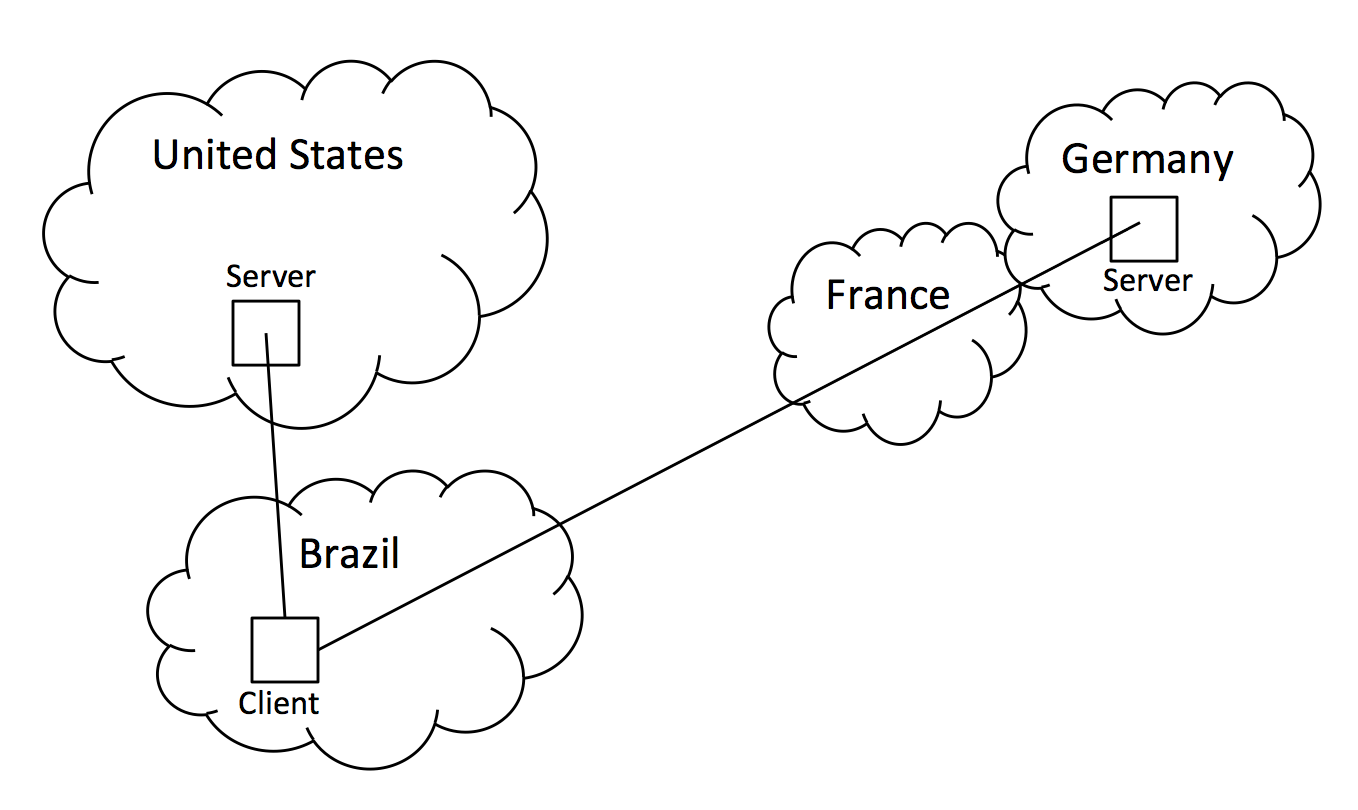
\includegraphics[width=.5\textwidth]{intro_fig}
\caption{A shorter path to a server in a country known for surveillance (U.S.), and a longer path to a georeplicated server in Germany.  The longer path may be more preferred by the client because it doesn't traverse a country with known surveillance practices.}
\label{fig:intro}
\end{figure}

This paper is organized as follows.  In the next section, we describe
our research goals, and the challenges in achieving them.  In
Section~\ref{datasets} we discuss how and where we collected our data.
We point out the advantages and disadvantages of existing datasets, and
justify our decision.  In Section \ref{measure}, we design and execute a
measurement study on the country-level paths of Brazil's Internet.  We
describe our methodology, as well as results that show which countries
Brazil's Internet traffic is traversing.  Next, Section
\ref{architecture} introduces \system{}, which allows Internet users, ISPs,
and Internet services to avoid specified countries, and therefore
circumvent surveillance.  Then we explain our implementation of \system{}
in Section \ref{implementation}.  In Section \ref{evaluation}, we
evaluate our system and proposed methods for how well they avoid any
given country.  We discuss how our system differs from others and
uniquely suits the purpose of country avoidance in Section
\ref{discussion}, we review related work in Section \ref{related}, and
conclude in Section \ref{conclusion}. 
